\section {Два корня внутри промежутка}

Расположение двух корней внутри промежутка (Вариант $I$) допускает границы четырёх типов:

\begin {enumerate} [labelindent=\parindent, leftmargin=*]
    \item {$[\alpha, \beta]$}
    \item {$[\alpha, \beta)$}
    \item {$(\alpha, \beta]$}
    \item {$(\alpha, \beta)$}
\end {enumerate}

Особый случай для границ типов 1--3 "--- это попадание одного корня уравнения $f(x) = 0$ на
включённый конец промежутка, а второго "--- либо внутрь промежутка, либо на его включенную границу.

\subsection {Границы второго типа}

Например, особому случаю второго типа границ будет соответствовать следующая ситуация:

\begin {figure} [h]
    \begin {minipage} [t] {\linewidth}
        \centering
        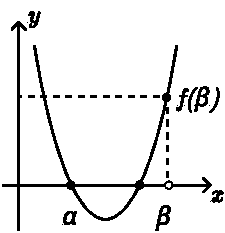
\includegraphics [width=0.3\linewidth] {images/image_01.pdf}
    \end {minipage}
\end {figure}

Чтобы обработать этот случай, необходимо рассмотреть прохождение параболы $y = f(x)$ через точку
$\alpha$, то есть решить уравнение

\begin {equation*}
    f(\alpha) = 0
\end {equation*}

Если полученное уравнение сводится к уравнению, которое вы умеете решать, то в результате получится
конечное число параметров $p$. Чтобы понять, какие параметры $p$ подходят, можно подставить каждое
значение в трёхчлен $f(x)$ и проверить, принадлежит ли второй корень уравнения $f(x)=0$ промежутку
$[\alpha, \beta)$. Это можно сделать с помощью теоремы Виета, так как один из корней уже известен
($x_1 = \alpha$), или проверкой соответствующих условий:

\begin {equation*}
    \begin {cases}
        \alpha < x_0 < \beta,
        \\
        a \cdot f(\beta) > 0.
    \end {cases}
\end {equation*}

\subsection {Границы четвёртого типа. Общий случай}

Границы четвёртого типа исключают особые случаи и являются, вообще говоря, общим случаем:

\begin {figure} [h]
    \begin {minipage} [b] {\linewidth}
        \centering
        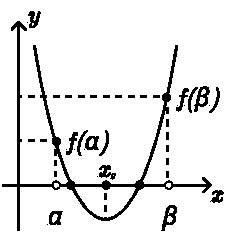
\includegraphics [width=0.3\linewidth] {images/image_02.pdf}
    \end {minipage}
\end {figure}

Чтобы оба корня были внутри интервала $(\alpha, \beta)$ необходимо выполнение следующих условий:

\begin {itemize}
    \item {существует 2 корня}
    \item {вершина параболы лежит внутри промежутка}
    \item {на концах промежутка значения квадратного трёхчлена положительны (с точностью до
    умножения на коэффициент $a$)}
\end {itemize}
получаем следующую систему:

\begin {equation*}
    \begin {cases}
        D > 0,
        \\
        \alpha < x_0 < \beta,
        \\
        a \cdot f(\alpha) > 0,
        \\
        a \cdot f(\beta) > 0.
    \end {cases}
\end {equation*}

Как уже говорилось, чтобы получить полное решение задачи, нужно объединить особые случаи с общим
решением.
